%%This is a very basic article template.
%%There is just one section and two subsections.
\documentclass{article}
\usepackage{geometry}
 \geometry{
 a4paper,
 left=20mm,
 top=20mm,
 }
\usepackage[latin1]{inputenc} %coding of writteninput %latin1 allows for Umlaute
\usepackage[T1]{fontenc}%vectorized fonts (cm-super package)
\usepackage[english]{babel}%some specifics of the german language
\usepackage{amsfonts, amsmath, amsthm, amssymb, mathabx, paralist}
\setlength{\parindent}{0em} 

 %Decisiontree
 \usepackage{tikz,forest}
 \usepackage{tikz}
\usetikzlibrary{arrows,shapes,snakes,automata,backgrounds,petri}
\usetikzlibrary{arrows.meta}

\usepackage{graphicx}
\usepackage{caption}
\usepackage{subcaption}

\usepackage{verbatim}%f�r txt datei

\usepackage{multirow}

\usepackage{ textcomp } %textrightarrow

\title{Homework 2}
\author{ Miriam Wagner\\373045}
\begin{document}
\maketitle

\tableofcontents
 	
%\mainmatter
\section{Introduction}
In this assignment I have to analyze for a financial institute data and make suggestions for the company. The event log is taken from the information system while it is running. 

All researches were done with ProM as ecpected from us. The data contains three types of activities (taken from the Assignment):

\begin{enumerate}
	\item Event names that start with "App\_" refer to status changes of applications. People make applications for a loan online.
	\item Event names that start with "P\_" refer to status changes of proposals, i.e. if the financial institute sees an opportunity to sell a loan to a customer, a proposal is sent to the customer.
	\item Events that start with "W\_" refer to activities performed by employees in the process, for example the call-center employees
\end{enumerate}

The data was analyzed in several steps to get a better idea of the process and to make recommendations. Firstly I had a look at the data itself, secondly I split the data in 3 seperate models to better understand the processes. Based on this I had a look at the proposal c-net and created my own lifecylce. In the next steps I had a look at the application and workflow lifecycle searching for bottlenecks and possible optimizationsteps.
Concluding I also explored the influence of the requested amount on the decisions taken, if there are employees having more influence on the outcome of a case and compared the thoughput times of nonapproved and approved cases.

\section{General insights about the data set}

The given data set is generated between 1st Oct 2011 0:38:44 (Saturday) and 14th Mar 2012 16:04:54 (Wednesday) and contains 13087 cases with 262200 events executed. One case contains minimal 3 events and maximal 175. In average 20.035 events.

There are 4366 different variants of cases. There are 36 different events possible 
"W\_Complete\_Application + COMPLETE" (9.141\%), "W\_Complete\_Application + START" (8.967\%), "W\_Quotations + COMPLETE" (8.763\%), "W\_Quotations + START" (8.545\%), "App\_Fully\_Submission + COMPLETE" (4.991\%), "App\_Incomplete\_Submission + COMPLETE" (4.991\%), "W\_Handeling\_Incomplete\_Dossiers + COMPLETE" (4.35\%), "W\_Handeling\_Incomplete\_Dossiers + START" (4.348\%), "W\_Validation + COMPLETE" (3.011\%), "W\_Validation + START" (3.01\%), "App\_Rejection + COMPLETE" (2.912\%), "W\_Complete\_Application + SCHEDULE" (2.811\%), "App\_Pre\_Acceptation + COMPLETE" (2.81\%), "P\_Initiation + COMPLETE" (2.681\%), "P\_Selection + COMPLETE" (2.681\%), "P\_Sending + COMPLETE" (2.681\%), "W\_Quotations + SCHEDULE" (2.53\%), "W\_Handling\_Leads + COMPLETE" (2.249\%), "W\_Handling\_Leads + START" (2.249\%), "App\_Acceptation + COMPLETE" (1.95\%), "W\_Validation + SCHEDULE" (1.916\%), "App\_Finalization + COMPLETE" (1.913\%), "W\_Handling\_Leads + SCHEDULE" (1.82\%), "P\_Cancellation + COMPLETE" (1.394\%), "P\_Returning + COMPLETE" (1.317\%), "App\_Cancellation + COMPLETE" (1.071\%), "W\_Handeling\_Incomplete\_ Dossiers + SCHEDULE" (0.909\%), "App\_Initiation + COMPLETE" (0.857\%), "App\_Approving + COMPLETE" (0.857\%), "App\_ Registration + COMPLETE" (0.857\%), "P\_Acceptation + COMPLETE" (0.855\%), "P\_Rejection + COMPLETE" (0.306\%), "W\_Fraud\_ Detection + COMPLETE" (0.103\%), "W\_Fraud\_Detection + START" (0.103\%), "W\_Fraud\_Detection + SCHEDULE" (0.047\%) and "W\_Changing\_Contact\_Details + SCHEDULE" (0.005\%).

The complete, start and shedule are more details about the state of the event. Just about the Workflow events I have more information about the state. 

All processes start in "App\_Fully\_Submission + COMPLETE" (100.0\%).

The processes can end in 13 different events:

"App\_Rejection + COMPLETE" (26.202\%), "W\_Validation + COMPLETE" (20.975\%), "W\_Handling\_Leads + COMPLETE" (17.07\%), "W\_Complete\_Application + COMPLETE" (14.816\%), "W\_Quotations + COMPLETE" (9.849\%), "App\_Cancellation + COMPLETE" (5.005\%), "W\_Handeling\_Incomplete\_Dossiers + COMPLETE" (3.454\%), "P\_ Cancellation + COMPLETE" (2.132\%), "W\_Fraud\_Detection + COMPLETE" (0.436\%), "W\_Changing\_Contact\_Details + SCHEDULE" (0.031\%), "W\_Validation + START" (0.015\%), "App\_Registration + COMPLETE" (0.008\%) and "W\_ Quotations + START" (0.008\%).

What you already see here, is that the process not always ended like expected, because the log is taken from the running system. All the process ending with a start event are probably not done now. 


\begin{figure}[!htbp]
\centering
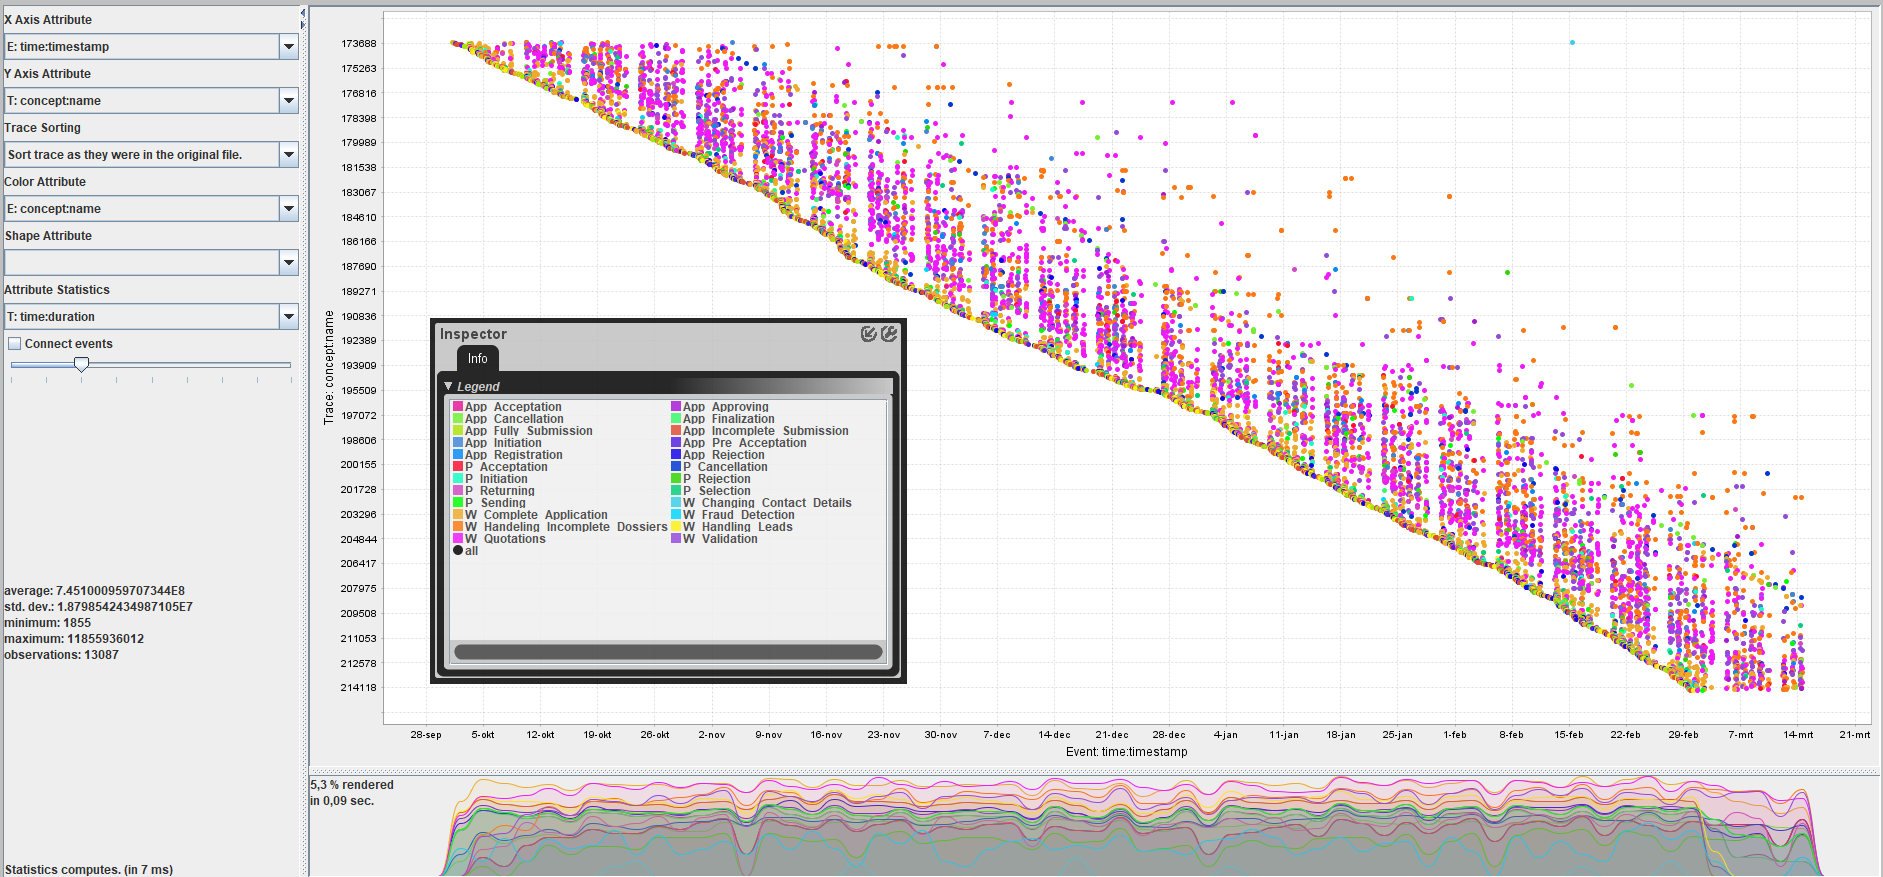
\includegraphics[width = 0.9\textwidth]{TotalDataDot.PNG}
\caption{Dotted chart of the data set}
\label{fig:WholeDat}
\end{figure}

Having a look at the whole data, figure \ref{fig:WholeDat} it can be seen, that there are just the following events executed at sundays: "W\_Complete\_ Application", "W\_Handling\_Leads", "App\_Incomplete\_Submission", "P\_Cancellation", "App\_Fully\_ Submission" and "App\_Rejection". Furthermore is there a constant input of new cases. The events are mostly executed the same amount of times just "W\_Fraud\_Detection" and "W\_Changing\_Contact\_Details" have really deeps and ups. What is not surprising, because both are outlier behavior actions.
\section*{Process Models}
%Providing process models is not enough because the process owner is diffident with any result which he/she is simply provided with. Therefore, he/she wants evidence of the goodness of these models. For this purpose, you should perform alignment-based conformance checking. Using the result of the conformance checker, you should motivate why the chosen models are better that any possible alternative (e.g. because of mediating fitness, precision, generalization and simplicity). For each model, also provide its textual description. 

\subsection*{The model of the application's lifecycle}
%filter on event names
%interactive data heuristic miner

\subsection*{The model of the proposal's lifecycle }

\subsection*{Combinded Model}
%Models that combine these two models into one showing the lifecycle of the application and the proposal together. Due to the high variability, you should discover one different model for each possible outcome, namely whether the application is finally rejected, cancelled or approved. 

\subsection*{C-net of the proposal process}
%Analyze the C-net of the proposal process and explain it. 

\subsection*{Own Petri net of the proposal process}
%Based on your analysis, create a Petri net of the proposal process by your own. For example, do not consider infrequent paths and also outlier behaviors. 

\subsection*{Analysis of the performance of Application and work process}
%Analyze the performance of Application and work process. What are the bottlenecks? What are your recommendations to the company to increase the performance of the process? 
\section{Further questions}
% 1. Are some decisions in any of the models driven by the application’s amount?
% 2. Are there clear indications that the same employees are always involved in cases that are
% declined, approved or cancelled?
% 3. The process owner would like to see a comparison of the throughput times between the nonapproved
% applications, i.e. those cancelled or rejected by the applicant, and the approved
% applications. In particular, he/she is interested in the time between the moment in which an
% application is submitted and when it is approved, compared with the time between the
% application is submitted and it is rejected or cancelled. 

\subsection{Are some decisions in any of the models driven by the application's amount?}
For answering this question I had a look at the dotted charts of the whole data set and the three filtered ones, "Filtered App", "Pdoubledfiltered", "Filtered Work". As x-axis I chose "C:Activity classifier" and y-axis "T:AMOUNT\_REQ". Also I sorted the traces by the "AMOUNT\_REQ". Just for the layout I changed the color to "C: Activity classifier".

\begin{figure}[!htbp]
\centering
\begin{subfigure}{0.49\textwidth}
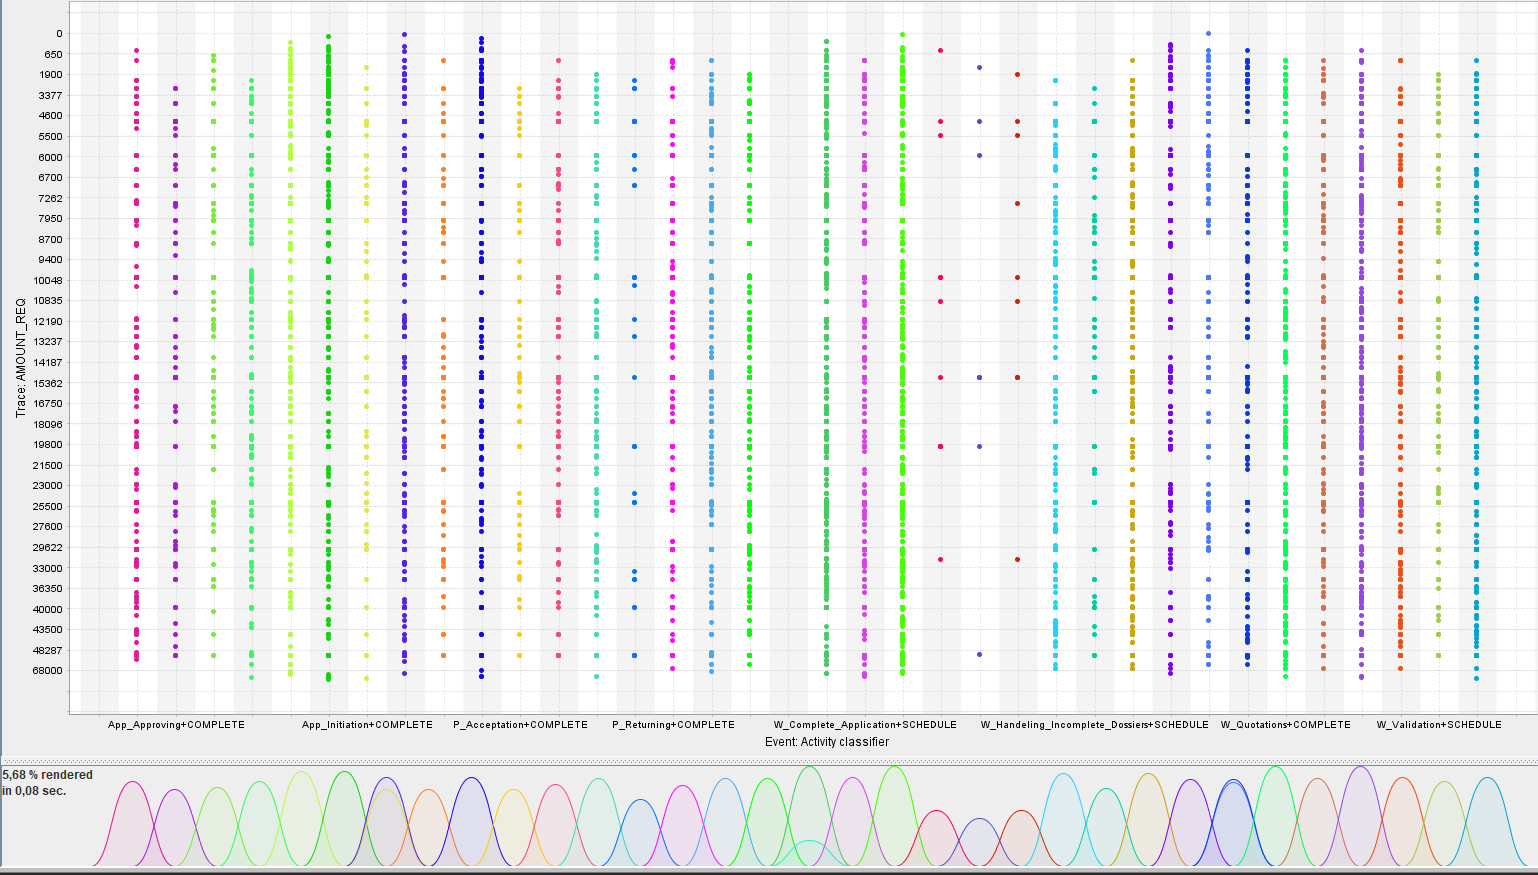
\includegraphics[width = 0.99\linewidth]{AmountRequ_All.PNG}
\caption{Whole data set}
\label{fig:AmounWhole}
\end{subfigure}
\begin{subfigure}{0.49\textwidth}
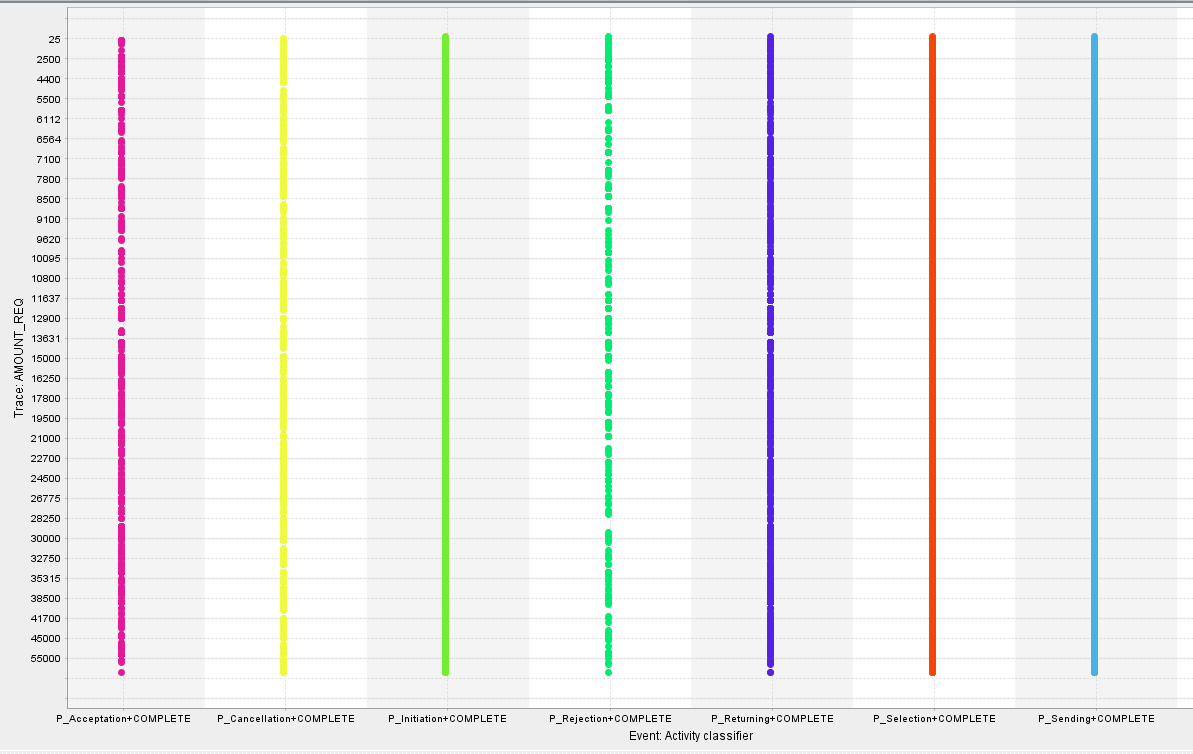
\includegraphics[width = 0.99\linewidth]{AmountRequ_P.PNG}
\caption{Proposal data set}
\label{fig:AmounP}
\end{subfigure}
\begin{subfigure}{0.49\textwidth}
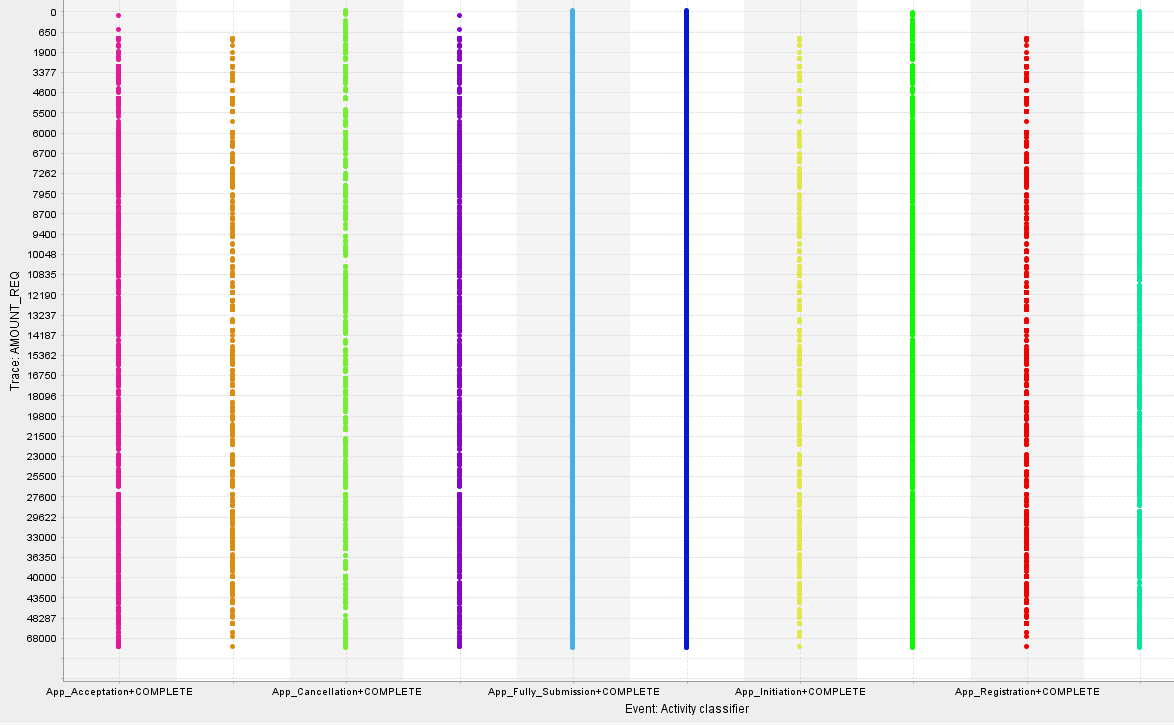
\includegraphics[width = 0.99\linewidth]{AmountRequ_App.PNG}
\caption{Application data set}
\label{fig:AmounApp}
\end{subfigure}
\begin{subfigure}{0.49\textwidth}
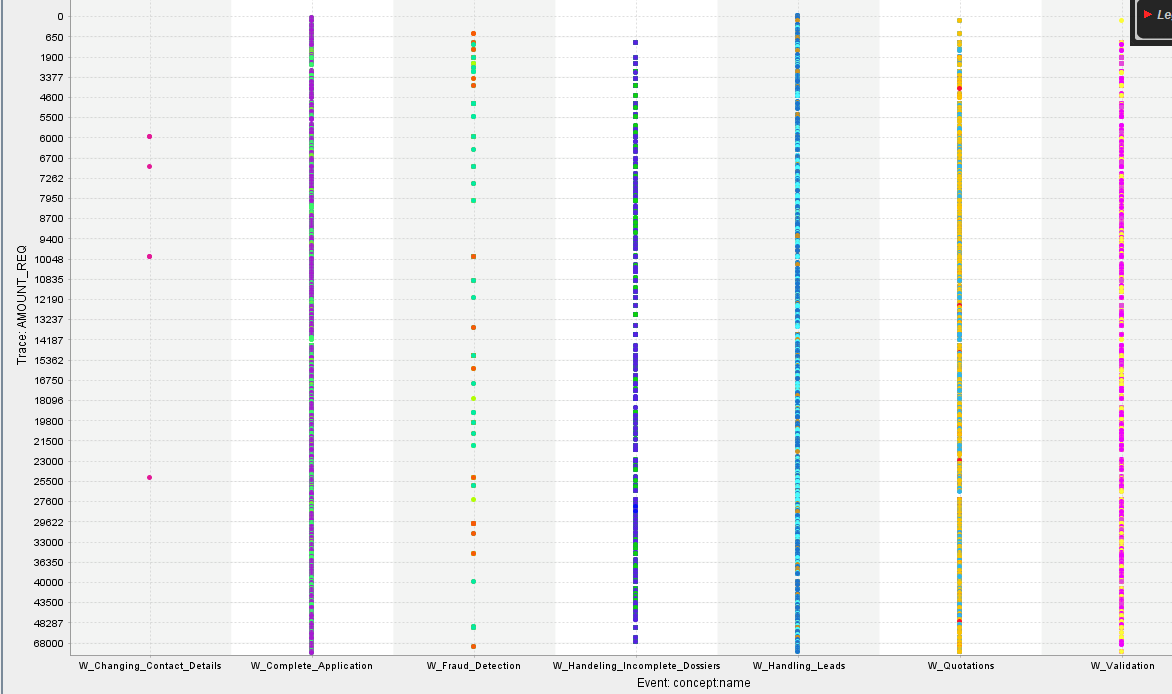
\includegraphics[width = 0.99\linewidth]{AmountRequ_Work.PNG}
\caption{Workflow data set}
\label{fig:AmounWhole}
\end{subfigure}
\caption{Dotted chart for the application's amount}
\label{fig:DotAmount}
\end{figure}

Figure \ref{fig:DotAmount} shows clearly, that there is \textbf{no correlation} between activity and requested amount. 

\subsection{Are there clear indications that the same employees are always involved in cases that are declined, approved or cancelled?}

For this question I concentrate on the application data set and filter it three time: "Filtered App with approv", where as end event just "APP\_Initation", "APP\_Registration" and "APP\_Approved" are possible as end event, based on the result of the 6th question before, where you can see, those three always happen together, "Filtered App with Rej", end event just "APP\_Rejected" and "Filtered App with Canc"

Those filtered data sets I used for the \textbf{Interactive Data aware Heuristic Miner}, where I chose resource in place of activity to create a model.

\subsubsection{Approved}

To see what are the main resources used I had a look at the c-net.
\begin{figure}[!htbp]
\centering
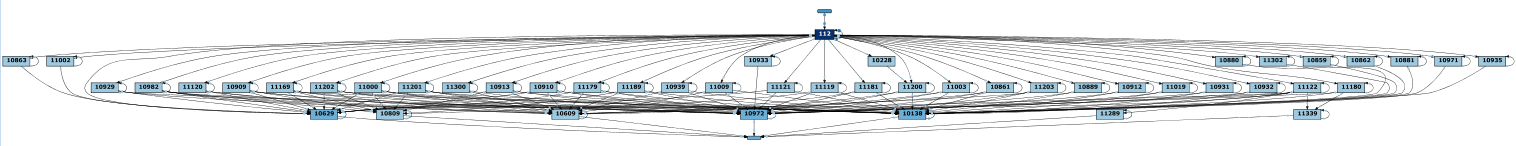
\includegraphics[width = 0.9\textwidth]{ApprovCnet.PNG}
\caption{Causal net of the approved application lifecyle without filtering}
\label{fig:CnetApprov}
\end{figure}

\begin{figure}[!htbp]
\centering
\begin{subfigure}{0.4\textwidth}
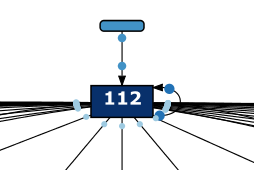
\includegraphics[width = 0.9\linewidth]{ApprovCnetBeginning.PNG}
\caption{Beginning of the traces}
\label{fig: CnetApprovBeg}
\end{subfigure}
\begin{subfigure}{0.4\textwidth}
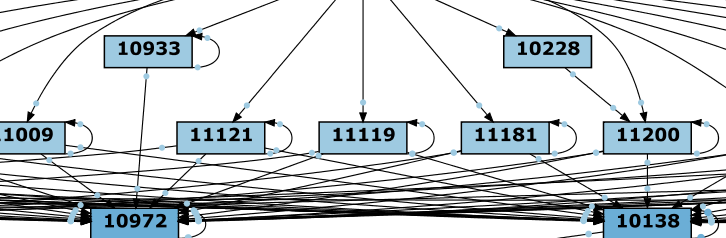
\includegraphics[width = 0.9\linewidth]{ApprovCnetMiddle.PNG}
\caption{Middle of the traces}
\label{fig: CnetApprovMid}
\end{subfigure}
\begin{subfigure}{0.9\textwidth}
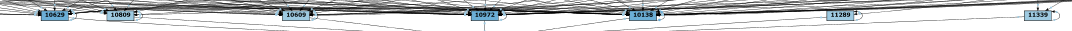
\includegraphics[width = 0.9\linewidth]{ApprovCnetEnd.PNG}
\caption{End of the traces}
\label{fig: CnetApprovEnd}
\end{subfigure}
\caption{Zoomed in the c-net}
\label{fig:CnetApprovZoome}
\end{figure}

There are three parts prominent, \ref{fig:CnetApprovZoome}:
\begin{enumerate}
	\item All traces start via \textbf{112}, \ref{fig: CnetApprovBeg}
	\item 2 resources, 10933 and 10228, just have two successors, \ref{fig: CnetApprovMid}
	\item 7 resources execute the last event, \ref{fig: CnetApprovEnd}
\end{enumerate}

\subsubsection{Rejected}

\begin{figure}[!htbp]
\centering
\begin{subfigure}{0.7\textwidth}
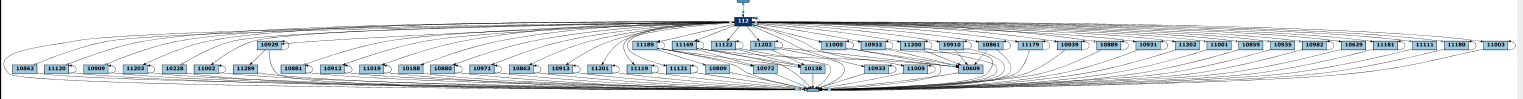
\includegraphics[width = 0.9\linewidth]{RejCNet.PNG}
\caption{Causal net of the reject application lifecyle without filtering}
\label{fig:CnetRej}
\end{subfigure}
\begin{subfigure}{0.2\textwidth}
\includegraphics[width = 0.9\textwidth]{RejCnetBeg.PNG}
\caption{Zoomed in the beginning of the c-net}
\label{fig:CnetRejZoome}
\end{subfigure}
\caption{Rejection resource c-net}
\label{fig:CnetRejto}
\end{figure}

Figure \ref{fig:CnetRej} shows the whole c-net and in \ref{fig:CnetRejZoome} it is more clear, that again \textbf{112} starts all traces.

\subsubsection{Cancellation} 

\begin{figure}[!htbp]
\centering
\begin{subfigure}{0.7\textwidth}
\includegraphics[width = 0.9\linewidth]{CancCNet.PNG}
\caption{Causal net of the cancellation application lifecyle without filtering}
\label{fig:CnetCanc}
\end{subfigure}
\begin{subfigure}{0.2\textwidth}
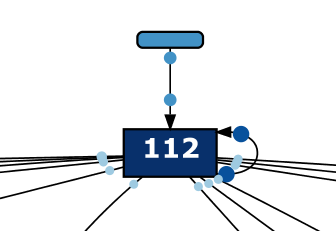
\includegraphics[width = 0.9\linewidth]{CancCnetBeg.PNG}
\caption{Zoomed in the beginning of the c-net}
\label{fig:CnetCancZoome}
\end{subfigure}
\caption{Cancellation resource c-net}
\label{fig:CnetCancto}
\end{figure}

Figure \ref{fig:CnetCanc} shows the whole c-net and in \ref{fig:CnetCancZoome} it is more clear, that again \textbf{112} starts all traces.

\subsubsection{Summary of those results}

So what gets pretty clear is that \textbf{112} decides over the next steps in the beginning. Having a look at the resources following it gets obvious, that different ressources work on the 3 sorts of traces. So it seems to depend on 112, which decision will be made.


\subsection{Comparsion of the throughput times}
%The process owner would like to see a comparison of the throughput times between the nonapproved applications, i.e. those cancelled or rejected by the applicant, and the approved
% applications. In particular, he/she is interested in the time between the moment in which an
% application is submitted and when it is approved, compared with the time between the
% application is submitted and it is rejected or cancelled. 

For this investigation I created a data set with the combination of rejected and cancelled traces, "Filtered App with rej and canc".

Then I looked the times up in the dotted chart like I did before.


\begin{figure}[!htbp]
\centering
\begin{tabular}{|c|c|c|c|}
\hline
& Minimum & Mean & Maximum \\ \cline{1-4}
Approved& $700910$ & $1.4393*10^9$ & $ 7419735534$      \\ \cline{1-4}
Rejected of cancelled  & $1855$ & $5.613*10^8$ & $7901736161$       \\ \cline{1-4}
\end{tabular}
\caption{Throughput times}
\label{tab:Throughtimes}
\end{figure}

In figure \ref{tab:Throughtimes} it can be clearly seen, that an approved traces takes 2.56 times so much time, than a rejected or cancelled trace. 

\section{Conclusion}
Recapping all results from the last parts I would say, that there a few points throughout the event, where it could be done better. There are 2 big bottlenecks in the process, which should be optimzied. Also the use of the resources could be optimized. The difference between the fastest trace is much faster than the slowest one, which should be analyzed in more detail for all process parts.

\end{document}
